\documentclass{article}
\usepackage{tikz}
\usepackage{caption}
\pagestyle{empty}

\begin{document}

\begin{figure}[ht]
    \centering
    \captionsetup{type=figure} % 不显示标题
    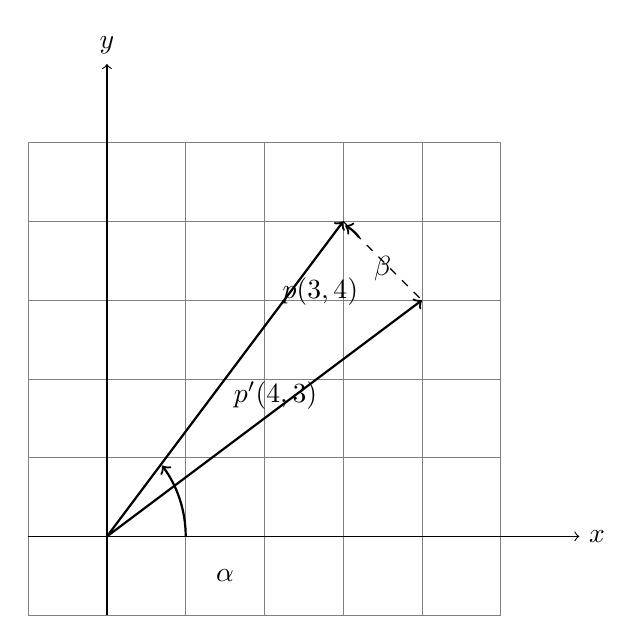
\begin{tikzpicture}
        \draw[very thin, gray] (-1,-1) grid (5,5);

        % 绘制坐标系
        \draw[->] (-1,0) -- (6,0) node[right] {$x$};
        \draw[->] (0,-1) -- (0,6) node[above] {$y$};

        % 绘制初始线段和变化后的线段
        \coordinate (start) at (0,0);
        \coordinate (end) at (3,4);
        \coordinate (changed_end) at (4,3);

        \draw[->, thick] (start) -- (end) node[pos=0.7, above right] {$p(3, 4)$};
        \draw[->, thick] (start) -- (changed_end) node[pos=0.7, below left] {$p'(4, 3)$};

        % 标记角度 alpha 和 belta
        \draw[dashed] (0,0) -- (4,0);
        \draw[->, thick] (1,0) arc[start angle=0,end angle=36.87,radius=1.5cm];
        \node at (1.5,-0.5) {$\alpha$};

        \draw[dashed] (3,4) -- (4,3);
        \draw[->, thick] (3.2,3.8) arc[start angle=36.87,end angle=63.13,radius=0.5cm];
        \node at (3.5,3.4) {$\beta$};
    \end{tikzpicture}
    \label{fig:changed_segment}
\end{figure}

\end{document}
